\documentclass{article}
\usepackage{amsmath} % equation, align, matrix, *, &, \\, \left, \right
\usepackage{graphicx} % figure
\usepackage{subcaption} % subfigure
\usepackage{comment} % To comment
\usepackage{hyperref} % To hyperlink and ref
\usepackage{enumitem} % To list
%\usepackage[ngerman]{babel}
\usepackage[utf8]{inputenc}
\usepackage{wrapfig}
\usepackage{ulem}
\usepackage[backend=bibtex,style=numeric]{biblatex}
\usepackage{subfiles} %multifile latex projects
\usepackage{multirow}
\usepackage{booktabs}
\usepackage{csquotes}
\usepackage[section]{placeins}
\usepackage{color,soul}

%\usepackage{fontspec}
\graphicspath{{images/}{../images/}}

\bibliography{lib} 

\title{IoT Project: \\Height / capacity monitor}
\author{Grupo K: \\ Tim Reiprich \\ Tegshigzugder Otgonbayar \\ Luca Maltagliati}

\begin{document}

\pagestyle{plain} \pagenumbering{gobble} %hide page numbers

\maketitle
% \section{}
% \subsection{}
% \subsubsection{}

% \paragraph{}
% \subparagraph{}

\newpage

\pagenumbering{arabic} %show page numbers in arabic
\tableofcontents % from the section headings
\newpage

% \listoffigures \listoftables
% \newpage

\section{Introduction}

In the project of the course Internet of Things we are to implement a device, that is capable of executing a specific task in a given environment. For this project we chose from the possible project ideas the height and capacity monitor. The selection of the idea was simple for us, as we were interested in a project, that has a practical usage in reality. There are certain sceneries such as: for example, in a household with children, to monitor the height and capacity of kitchen or restroom sinks. So in the case, that the water runs over, to turn it off or to notify the family. Also in industrial area cases such as: monitoring the amount of liquid to be poured in a container.

Our task was to develop such a device and document the procedures. During this project we worked intensively with the Arduino IDE and Node-RED.

\section{General description}

Our project focuses on the measurement of containers holding some sort of liquid. Based on the volume of these containers alarms are sent to the users to notify them about the amount. To accomplish this, a sensor will be used, that determines the height of the liquid in the container. Furthermore an upper and a lower threshold will be set by the user. If a threshold is exceeded, an alarm, in form of a LED at the sensor and a virtual LED in Node-RED, will trigger.

\subsection{Hardware scheme}

\begin{figure}[]
  \hspace{-1.5cm} \includegraphics[scale=0.325]{images/circuit3.png}
  \caption{Draft of the scheme}
  \label{scheme}
\end{figure}

In this part we will discuss the basic scheme of the system hardware. The main components are:
\begin{itemize}
\item a computer as central server
\item the sensors
\item a webpage
\end{itemize}
The sensors must be able to connect to the server via a Wi-Fi connection. For this we assume a robust connection, that is available in the given environment. The homepage is hosted on the central server and is the main way to interact with the system for the end-user. Theoretically it should be straightforward to expand the system, so it functions with numerous amounts of height sensors as shown in the figure \ref{scheme}. To only showcase and due to the restriction of available components we will implement with a single sensor. This sensor communicates with the central server.

\subsection{Sensor}
To measure the height of the liquid we use an ultrasonic sensor called Ultrasonic Sensor Module HC-SR-04 by Robokart. We have chosen this approach because it is a simple and cheap way to sense the proximity and detect the capacity level. The sensor is connected to a microcontroller which
collects data and via a Wi-Fi connection sent to the central server.

Each container will contain a microcontroller that is at least connected to one sensor, as shown in the figure \ref{sensorWithArduino}. Specified heights of minimal and maximal volumes can be set dynamically, depending on various factors such as: the position of the container, the probability of its usage and the type of liquid.

\begin{figure}[]
	\centering
  \includegraphics[scale=0.5]{sensorAndArduino.jpg}
  \caption{Example of a sensor connected to a microcontroller}
  \label{sensorWithArduino}
\end{figure}

\subsection{Central server}

Through a LAN or WLAN network, to which the controllers and central server are
connected, the microcontrollers will communicate with the central server by sending the measurements of the liquid heights continuously. Then the central server will perform checks on the current set thresholds of the user. If necessary it will show the alarm on the homepage and send the signal to the microcontroller, which are connected to the sensor. So the alarm, in form of the connected LEDs, will be triggered as well. This procedure and the corresponding homepage were configured in Node-RED.

\section{Project}

The first step of the project was to research about other similar projects and
to identify platforms, programming languages and frameworks, to choose the best suited for our case. The connection between the devices plays a crucial role, so we needed to know what kind of protocols are crucial. In the next step we planned the structure of the system and began to familiarize with
the tools we wanted to use. After the planning we implemented the system and tested it to remove possible errors.\par

\subsection{Components}
Here we have the components used for the project and their usages. These are:
\begin{itemize}
\item NodeMCU DevKit v1.0 development board (ESP8266) - we will use the
  microcontroller to connect to the sensor. It will collect and send data to the broker and
  receive parameters to light the warning LEDs correctly.
\item Ultrasonic proximity sensor (digital/analog output module) - the main
  sensor to measure the distance to the liquid
\item Power source for the microcontroller and sensor (batteries, solar panel or
  similar source)
\item Smaller materials:
	\begin{itemize}
  \item cables - to connect sensor, microcontroller and LEDs
  \item breadboard - to connect sensor, microcontroller and LEDs
  \item LEDs - to signal an alarm
	\end{itemize}
\end{itemize}

\subsection{Wiring scheme}
For the implementation of the system we use the setup shown in the figure \ref{schema_bb}. We use  batteries to power the system, which makes it more flexible to use. However it results in downtimes, when the batteries have to be changed. For a more stable system the batteries can be exchanged with a permanent connection to a power socket.

\begin{figure}[]
	\centering 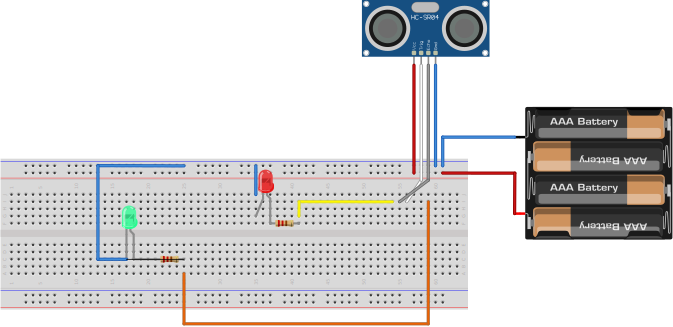
\includegraphics[scale=0.4]{images/schema_bb.png}
	\caption{Hardware scheme}
	\label{schema_bb}
\end{figure}

\subsection{Flow chart of system functionality}
After the wiring scheme the flow of execution was planned. As shown in the figure \ref{flowChart} the parameters, regarding the thresholds and the height of the basket, have to be set by the user at the start. Afterwards the system begins a loop. It is only stopped through a disconnect from the MQTT broker or through a loss of power supply.

\begin{figure}[]
		\center \includegraphics[scale=0.6]{flowChart.png}
		\caption{Flow chart of the system}
		\label{flowChart}
\end{figure}

\subsection{Node-RED}
This section covers the parts of the project running on the central server, which
mainly includes the homepage created with Node-RED. The flow of the project is shown in the figure \ref{flowScheme}. The simple user interface is shown in the figure \ref{inteface_offline}. The flow consists of four input elements located on the left side. Located in the middle of the flow, there are nodes, which transform the input data. On the right side the output nodes are located.\par

\paragraph{Input nodes}\mbox{}

Three of the four input nodes are simple text nodes. Through which the user can set perspectively
the basket height, the lower threshold and the higher threshold. All three can be changed at any point, also if the system is running. This may be needed in cases such as: the liquid in the basket has been changed and due to a higher density the basket can't hold as much as before, the sensor is used in different basket. The basket height should be set because the ultrasonic sensor measures
faulty values from time to time. With the basket height these values can be filtered and prevent the
microcontroller from sending them to the MQTT broker.

The fourth input node receives MQTT messages from the MQTT broker. It is subscribed to the topic \enquote{distance}, to which the microcontroller publishes the measured distance.

\paragraph{Transforming and output nodes}\mbox{}
\label{sec:json}
The function node \enquote{Thresholds} checks if the user given
thresholds are valid. This means it checks if the lower threshold is lower or
equal to the higher threshold and vice versa. In these cases the
new values for lower and higher threshold are stored in \verb|conext.low| and
\verb|context.high|. The node returns 
\verb|{payload: {upper: context.high, lower: context.low}}|, which is used by the
two connected text nodes on the right side to show the user the currently set thresholds on the homepage.

The function node \enquote{Threshold Check} does the same checks as the previously discussed node and also stores the current threshold values in a similar manner.  Additionally it also stores the last measured distance and uses it to check if one of the two thresholds is surpassed. In the end the object \verb|{payload: {highLed: <boolean>, lowLed: <boolean>,| \verb| basketHeight:| \\
\verb|context.basket}}| is returned where the property 
highLed or lowLed is respectively set to \enquote{true} if the corresponding
threshold is surpassed. The last property always contains the current set
basket height. This is needed because the ultrasonic sensor returns abnormal values time to time. So we use the \verb|basketHeight| to filter the distance measurements higher than the height of the basket as these measurements are not possible and false. Afterwards this object is published to the topic
\enquote{threshold} as a JSON using MQTT. The microcontroller is subscribed to
this topic and uses the received values to turn its connected LEDs on or off and
to filter abnormal measured distances.\par
Besides that the returned object of the node \enquote{Threshold Check} is also
used as input for the function node called \enquote{filterLow}. It simplifies
the input and returns the object \texttt{\{payload: "high"|"low"|"between"\}}
where the value is chosen depending on the object given as input. We used this
so we can simply check for received string in the LED nodes afterwards in the
flow to determine if the LEDs have be turned off or on.\par
Finally the two output nodes on the top are used to show the measured
distances. The text node just shows the last measured distance in centimetres.
The node called \enquote{Distance} is a graph of the measured distances which
enables the user to see the tendencies in the liquid level and act before
the critical thresholds are exceeded.

\paragraph{User interface}\mbox{}
The user interface, shown in the figure \ref{inteface_offline}, is structured in three parts. On
the left the current status of the system is shown meaning the current
parameters of basket height, lower threshold and higher threshold. Also it contains three
status LEDs signalizing if one of the thresholds is surpassed or if the system
is in a non-problematic state (shown by the green LED names \enquote{normal}
being turned on).\par
In the middle the measurements are shown. This part consists of the last measured
distance and a graph showing the changes during the last measurements. These
values can only be seen if a microcontroller with an ultrasonic sensor is
publishing its data. Otherwise the graph is blank and the message
\verb|desconnectado| is shown instead of a measurement.

The part on the most right contains the nodes that allow user input. Through these the
user can set the basket height, lower threshold and higher threshold. This can happen
dynamically at any time. The changes will be published to the MQTT broker. Therefore the microcontroller publishes each time a value is changed or a measurement arrives.

\begin{figure}
	\hspace{-1cm}
	\includegraphics[scale=1.2]{images/flowScheme.png}
	\caption{Node-Red: Scheme of flow}
	\label{flowScheme}
\end{figure}

\begin{figure}
	\centering \includegraphics[scale=0.2]{images/interface_offline_2.png}
	\caption{Node-RED: Interface offline}
	\label{inteface_offline}
\end{figure}

\newpage

\subsection{Micro controller program}

In this part we will discuss the source file of the micro controller programs and its main methods. The code is contained in the source file \texttt{project.ino}, compiled and sent to the \texttt{ESP8266WiFi} microcontroller using \texttt{Arduino IDE}.

\paragraph{Communication with the sensor}\mbox{}

The logic of the distance measurement is implemented in the \verb|loop()|
function. Every half a second the measurement is done and published on the
\texttt{MQTT} topic. Since there is no need to publish additional information, the
data is published as a simple plain text, containing only the number with the
measurement or a string with an error message.

We are using an ultrasonic sensor. First we ensure the sensor is at low, then we
send a 10 milliseconds-long pulse and measure the time passed.

The function used to interact with the sensor is
\verb|digitalWrite(trigPin,flag)|,
where \texttt{trigPin} is the identifying number pin on the
microcontroller to which the trigger Pin of the sensor is connected to, as shown in the \ref{schema_bb}, and \texttt{flag} can be either \texttt{LOW} or \texttt{HIGH}, depending if we want
to trigger on or off the ultrasonic sensor. The distance is calculated with the formula:

\begin{equation}
\mathit{Distance} = \frac{\mathit{Time}/2}{29.1}
\end{equation}

\paragraph{Communication with the base station}\mbox{}

The \verb|callback()| function is invoked every time new data is published on
the topic. In particular, it is programmed to receive the \texttt{JSON} payload
described in the previous subsection \ref{sec:json}; we used the
\texttt{JSON} parsing library \texttt{ArduinoJson.h} to be able to de-serialize
it. The payload is de-serialized and the corresponding LEDs are turned off or on,
based on threshold trespassing information. Also the max height of the basket
can be set this way.

We also check the validity of the received \texttt{JSON}, debugging an error
message in case of syntax errors in the payload.

\paragraph{Additional functions}\mbox{}

The functions \verb|reconnect()| and \verb|setup_wifi()| check and/or establish
the connection to the Wi-Fi network. \texttt{reconnect()} is always called at the
start of every \texttt{loop()} call, to ensure the micro controller is connected at all times.

\newpage

\section{User manual}

\subsection{Setup}
The system can be set up in a few simple steps. The main prerequisite for a successful setup is a stable Wi-Fi connection over which the MQTT messages can be sent to and received from the MQTT broker. The login has to be configured in the code for the microcontroller as well as for the Node-RED homepage.\par 
Afterwards the microcontroller has to be connected to a power source and the ultrasonic sensor has to be fixed to the top of the container in which it's used pointing downwards towards the liquid stored in the basket. The rest of the hardware should be placed outside of the basket to prevent possible damage from the liquid and to make the warning LEDs easily visible.\par 
As soon as the microcontroller is connected to a power supply it tries to connect to the given Wi-Fi connection. If this is successful, it starts measuring the height and sending the data to the MQTT broker. When Node-RED is running on the central server hosting our homepage, it will start communicating with the MQTT broker as soon as the receiving and sending node are configured using the correct credentials.\par 
Once this initial setup is done the system should be running and the thresholds and the basket height can be set and dynamically changed to use the full spectrum of features.\par 
In case the microcontroller disconnects from the MQTT broker unexpectedly the message \verb|Desconectado| is shown instead of the last measured distance. In this case the established connection should be checked as well as the microcontroller at the basket because it may have lost power. In case the error is more complex, the Arduino IDE can be used as the system does extensive logging.

\subsection{Power Consumption}
During the class we measured the power consumption of the system. The
measurement happened over a duration of $8.3$ seconds and the results can be
seen in the figure \ref{chart_power}.\par
As seen in the graph the start-up lasted around 3 seconds. In the
beginning of it there are several spikes in power consumption. They could be the
result of initial processes but we do not know exactly what is going on the inside of
the ESP module. During $2.5$ and $3$ seconds there is a generally higher power
consumption without high spikes. It can be explained that this is the period of time during which
the ESP tries to establish a Wi-Fi connection. Due to constant package traffic
it could result in a higher consumption.\par
Afterwards there are a lot of spikes in power consumption which could have
happened because the microcontroller periodically sends and receives data from
the sensor, which is sent together with the other packages via Wi-Fi connection. Another possibility is if the connected LEDs are turned on or off, but this is hard to
tell given the sample.\par

If we want to minimize the power consumption of the system, we could lower
the frequency of measurements performed by the sensor. Therefore the
frequency of data exchange between the MQTT broker and the microcontroller lowers. Furthermore if the LEDs connected to the microcontroller are not needed, because perhaps they are not
visible or not important for the basket. Then they can be removed, so that the
system is more efficient.

\begin{figure}[]
\centering \includegraphics[scale=0.5]{images/chart.png}
\caption{graph of power consumption (until 8 seconds after start-up)}
\label{chart_power}
\end{figure}

\section{Summary}
In this project we have implemented a working system, which is able to monitor the height and capacity of a container. This document discusses the steps of our project and its functional details. Through this project we were able to learn a lot of different tools and methods to develop such a system. There are many advantages of using IoT devices in the daily life and it will be exciting to see, how it will develop further.

In the future it would be interesting to study the capability of interconnecting with other
devices and creating a more broad network of devices. It is very well imaginable, that the future homes and workplaces will be packed with IoT technology.

\end{document}
